\section{论文工作是否按预期进行、目前已完成的研究工作及结果}
\subsection{论文工作是否按预期进行}
本毕设课题工作一共分为三个部分。第一,将VNF-FG扩展问题建模为整数线性规划(ILP)模型,在合理的问题规模下找到最优解。第二,为响应新的租户需求,在满足对原始服务图的影响最小化约束的前提下,设计特征分解算法扩展先前已经部署的VNF-FG。特征分解算法通过实现加权图之间的最优匹配来解决VNF-FG扩展问题。第三,编程实现所设计的扩展算法,并在三个评价指标上与最优解进行比较。开题报告中的进度安排如表~\ref{table:1}所示。\par
\begin{table}[htbp]
    \centering
    \caption{进度安排表}
    \label{table:1}
    % \hspace{0.5cm}
    \begin{tabular}{p{40pt}p{230pt}p{130pt}}
        \toprule
        序号&研究内容&起止日期\\
        \midrule
        1	&查阅相关文献以及学术书籍,学习软件定义网络、网络功能虚拟化等基础知识	&2020.12.25-2021.01.15\\
        \midrule
        2	&学习VNF转发图的设计和扩展的相关知识	&2021.01.15-2021.02.01\\
        \midrule
        3	&将VNF-FG扩展建模为整数线性规划模型	&2021.02.01-2021.03.01\\
        \midrule
        4	&设计启发式算法扩展先前已经部署的VNF-FG,同时需要满足对原始服务图的影响最小化约束	&2021.03.01-2021.04.10\\
        \midrule
        5	&撰写中期报告,进行中期答辩	&2021.04.10-2021.04.15\\
        \midrule
        6	&仿真环境的设计与搭建,实现所设计的扩展算法并评估算法的性能	&2021.04.15-2021.05.10\\
        \midrule
        7	&总结研究结果,撰写论文	&2021.05.10-2021.05.26\\
        \bottomrule
    \end{tabular}
\end{table}

目前毕业设计按照开题报告中的进度计划,已经完成将VNF-FG扩展问题建模为整数线性规划模型和设计启发式算法扩展先前已经部署的VNF-FG,符合开题报告的进度计划。\par

\subsection{目前已完成的研究工作及结果}
\subsubsection{问题建模}
为对VNF转发图扩展问题进行建模,可以使用网络拓扑图来表示先前部署的VNF转发图、VNF扩展请求图和NFV物理基础设施图。因为VNF转发图和NFV物理基础设施图中的VNF节点具有不同的CPU容量、转发路径具有不同的带宽,所以需要定义若干约束条件。为了实现物理基础设施的负载均衡,也需要定义目标函数。\par
物理基础设施图被建模为一个无向加权图$G_p=(N_p,E_p)$,$E_p$是物理路径的集合,$N_p$是物理节点的集合。对于每个$N_p$集合中的物理节点k都具有两个特征。第一个特征是CPU处理能力,第二个特征是虚拟网络功能类型(或者物理网络功能PNF)。对于$E_p$集合中的每个物理链接e都具有可用带宽这个特征。以图~\ref{figure:1}为例,它包括两个物理网络功能设备、两个交换机以及一些互相连接的服务器。\par
\begin{figure}[H]
    \centering
    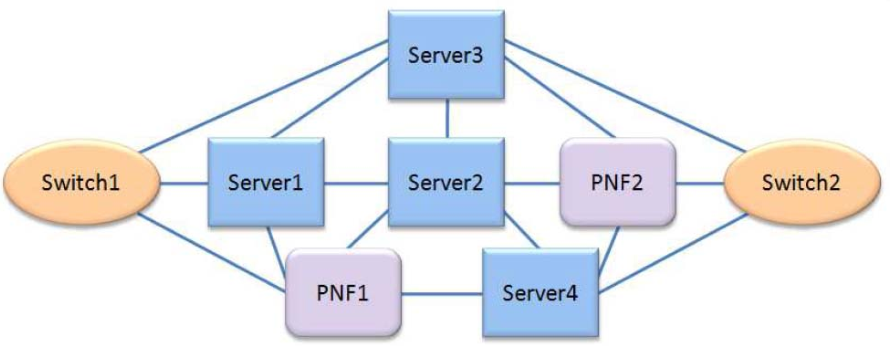
\includegraphics[width=.8\textwidth]{1.png}
    \caption{NFV物理基础设施图}
    \label{figure:1}
\end{figure}
类似地,客户的VNF请求转发图可以建模为$G_v=(N_v,E_v)$,其中$N_v$是请求图中虚拟节点集合,$E_v$是虚拟链路集合。对于每个虚拟节点都具有CPU处理能力和网络功能类型两个特征。对于每个虚拟链接都具有可用带宽的特征。图~\ref{figure:2}中描述了两个网络转发路径(NFP),转发路径是流量必须经过的有序VNF序列。\par
\begin{figure}[H]
    \centering
    
    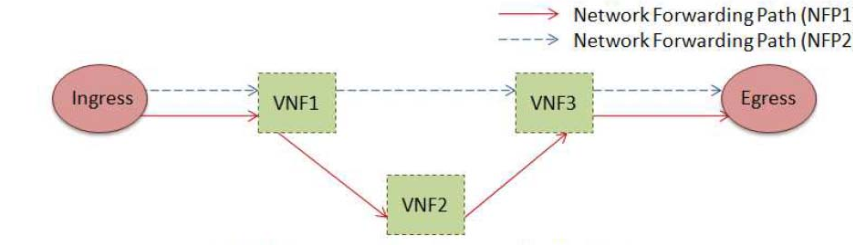
\includegraphics[width=.8\textwidth]{2.png}
    \caption{VNF请求转发图}
    \label{figure:2}
\end{figure}
为了更好地表示出VNF转发图的网络拓扑,可以从VNF转发图中推导出网络连接拓扑图(NCT)。网络连接拓扑图表示为$NCT_v=(N_v,E_v)$,是一个与$G_v$具有完全相同的节点和边集的无向加权图。惟一的区别是,网络连接拓扑图中的虚拟链接的可用带宽,是在$G_V$中通过该链接的所有VNF转发路径的带宽之和。图\ref{figure:3}为图\ref{figure:2}中的VNF请求转发图所对应的网络连接拓扑图。
\begin{figure}[H]
    \centering
    
    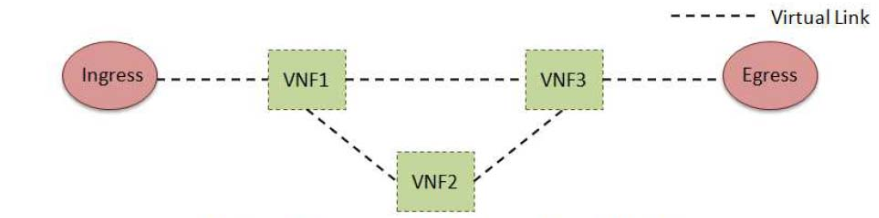
\includegraphics[width=.8\textwidth]{3.png}
    \caption{网络连接拓扑图}
    \label{figure:3}
\end{figure}

\subsubsection{约束条件和目标函数}
整数线性规划模型包括若干扩展算法必须满足的约束条件,用于找到合适的候选物理节点。为了通过优化求解器计算出扩展问题的最优解,需要提出与完整性约束条件相关联的目标函数。表~\ref{table:2}是对约束条件和目标函数中涉及变量的说明。
\begin{table}[H]
    % \linespread{1.25} 
    \setlength{\baselineskip}{1.2em}
    \setlength{\parskip}{0ex}
    \setlength{\parindent}{0pt}
    \centering
    
    \caption{约束条件涉及变量说明表}
    \label{table:2}
    % \hspace{0.5cm}
    \begin{tabular}{llp{40pt}p{230pt}}
        \toprule
        \textbf{变量符号} & \textbf{变量描述}\\
        \midrule
        $CPU_k$&物理节点k剩余计算容量\\
        \midrule
        $m_i,m_j$&VNF节点i和j的初始放置位置\\
        \midrule
        $P_{k_i,k_j}$&物理节点$k_i$和$k_j$之间的物理路径\\
        \midrule
        $\mathcal{C}$&物理节点集合\\
        \midrule
        $\mathcal{P}$	&物理路径集合\\
        \midrule
        $min_{CPU}$&$\mathcal{C}$中的最小CPU容量\\
        \midrule
        $BW_e$&物理链路e的剩余链路带宽\\
        \midrule
        $\delta_{ep}$&表示物理链接$e\in E_p$是否属于路径$P_{k_i,k_j}\in \mathcal{P}$: $\delta_{e p}=1\Leftrightarrow e\in \mathcal{P}$\\
        \midrule
        $N_v^{new},E_v^{new}$&扩展请求中的VNF节点集合,以及它们之间的链接的集合\\
        \midrule
        $N_v^{old},E_v^{old}$&旧VNF-FG请求中的VNF节点集合,以及它们之间的链接的集合\\
        \midrule
        $cpu_i$&虚拟节点i所需要的计算容量\\
        \midrule
        $bw_{e_{ij}}$&虚拟节点i和j之间的链路带宽\\
        \midrule
        $x_{ik}$&此变量为二元变量,表示VNF节点i是否放置到物理节点k上\\
        \midrule
        $y_{e_{ij}},P_{k_i,k_j}$&此变量为二元变量,表示虚拟链路$e_{ij}$是否会放置到物理路径${P_{k_i,k_j}}$\\
        \bottomrule
    \end{tabular}
\end{table}



旧节点映射约束:该约束用来维护旧VNF节点的初始映射位置。
\begin{equation}
    x_{i m_{i}}=1,\quad \forall i \in N_{v}^{\text {old}}
\end{equation}\par
旧链路映射约束:该约束用来维护旧虚拟链路的初始映射位置。
\begin{equation}
    y_{e_{i j}, P_{m_{i}, m_{j}}}=1,\quad \forall e_{i j} \in E_{v}^{\text {old }} 
\end{equation}\par
新节点映射约束:确保每一个新的VNF节点都能映射到一个物理候选节点,同时VNF组件不能拆分。
\begin{equation}
    \sum_{k \in \mathcal{C}} x_{i k}=1,\quad \forall i \in N_{v}^{\text {new }}
\end{equation}
\begin{equation}
    x_{ik}= \begin{cases}
        1,\quad \text{if the VNF i is hosted on the substrate node k}; \\
        0,\quad \text{otherwise}.
    \end{cases}
\end{equation}\par

CPU可用容量约束:确保VNF节点所放置物理节点的CPU可用容量大于等于该VNF节点的CPU容量。
\begin{equation}
    \sum_{i \in N_{v e w}^{\text {new }}} cpu_{i} \times x_{i k} \leq CPU_{k},\quad \forall k \in \mathcal{C} 
\end{equation}\par
新链路映射约束:如果虚拟链接的两端节点都是新的VNF节点,那么需要设置一个约束确保该链路能够被放置。
\begin{equation}
    \sum_{k_{i} \in \mathcal{C}} \sum_{k_{j} \in \mathcal{C}} y_{e_{i j}, P_{k_{i}, k_{j}}}=1,\quad \forall e_{i j} \in E_{v}^{\text {new }}, \forall i, j \in N_{v}^{\text {new }} 
\end{equation}
\begin{equation}
    y_{e_{i j}, P_{k_{i}, k_{j}}}=\left\{\begin{array}{ll}
        1, & \text { if the virtual link } e_{i j} \text { is mapped to physical path } P_{k_{i}, k_{j}} \\
        0, & \text { otherwise. }
        \end{array}\right.
\end{equation}\par
如果虚拟链接的源节点是旧节点、目的节点是新节点,那么需要满足以下约束。
\begin{equation}
    \sum_{k_{j} \in \mathcal{C}} y_{e_{i j}, P_{m_{i}, k_{j}}}=1,\quad \forall e_{i j} \in E_{v}^{\text {new }}, \forall i \in N_{v}^{\text {old }}, \forall j \in N_{v}^{\text {new }}
\end{equation}\par
如果虚拟链接的源节点是新节点、目的节点是旧节点,那么需要满足以下约束。
\begin{equation}
    \sum_{k_{i} \in \mathcal{C}} y_{e_{i j}, P_{k_{i}, m_{j}}}=1,\quad \forall e_{i j} \in E_{v}^{\text {new }}, \forall i \in N_{v}^{\text {new }}, \forall j \in N_{v}^{\text {old }} 
\end{equation}\par
带宽约束:物理路径上的每个物理链接的剩余可用带宽不能小于被放置在该路径上的所有虚拟链接的带宽要求的总和。
\begin{equation}
    \sum_{e_{i j} \in E_{v}^{\text {new }}} b w_{e_{i j}} \times y_{e_{i j}, P_{k_{i}, k_{j}}} \times \delta_{e p} \leq B W_{e},\quad \forall e \in P_{k_{i}, k_{j}}, \forall P_{k_{i}, k_{j}} \in \mathcal{P}
\end{equation}\par
节点和带宽约束:当$VNF_i$映射到物理候选节点$k_i$时,对于每个以$VNF_i$开始的虚拟链路$e_{ij}$都必须找到一个物理路径$P_{ki,kj}$来放置该虚拟链路.
\begin{equation}
    \sum_{k_{j} \in \mathcal{C}} y_{e_{i j}, P_{k_{i}, k_{j}}}=x_{i k_{i}},\quad \forall e_{i j} \in E_{v}^{\text {new }}, \forall k_{i} \in \mathcal{C}
\end{equation}\par
节点和带宽约束:当$VNF_j$映射到物理候选节点$k_j$时,对于每个以$VNF_j$开始的虚拟链路$e_{ij}$都必须找到一个物理链路$P_{ki,kj}$来放置该虚拟链路。
\begin{equation}
    \sum_{k_{i} \in \mathcal{C}} y_{e_{i j}, P_{k_{i}, k_{j}}}=x_{j k_{j}},\quad \forall e_{i j} \in E_{v}^{\text {new }}, \forall k_{j} \in \mathcal{C}
\end{equation}\par
节点分离约束:该约束要求所有VNF节点必须分开放置在不同的物理节点上, 原因包括安全问题、租户需求等等。
\begin{equation}
    x_{i k}+x_{j k} \leq 1,\quad \forall i, j \in N_{v}^{\text {new }}, \forall k \in \mathcal{C}
\end{equation}\par
目标函数:为了实现物理基础设施的负载均衡,目标函数应该倾向于选择剩余容量最多的物理节点和物理链接。$min_{CPU}$是物理候选节点中CPU计算容量的最小值,该最小值作为一个归一化因子,使算法尽可能选择那些拥有更多剩余计算能力的物理节点。
\begin{equation}
    \begin{aligned}
        \mathbb{Z}=&\left(\sum_{i \in N_{v}^{n e w}} c p u_{i} \times\left(\sum_{k \in \mathcal{C}} \frac{C P U_{k}}{\min _{C P U}} \times x_{i k}\right)\right) \\
        &+\left(\sum_{e_{i j} \in E_{v}^{n e w}} b w_{e_{i j}} \times\left(\sum_{k_{i} \in \mathcal{C}} \sum_{k_{j} \in \mathcal{C}} y_{e_{i j}, P_{k_{i}, k_{j}}}\right)\right)
    \end{aligned}
\end{equation}\par

   
\subsubsection{Umeyama特征分解算法}
为了解决VNF的放置问题,可以使用Umeyama的特征分解方法来实现加权图之间的最优匹配,然后基于匈牙利算法来提取映射结果。\par
加权图匹配问题是指在两个加权图之间寻找最优匹配的近似解。求解该问题的方法是在两个加权图之间找到一个映射函数,同时最小化两个图之间的相似距离度量。Umeyama算法通过对加权图的邻接矩阵进行特征分解,计算出两个特征向量矩阵的绝对值的乘积,然后使用匈牙利算法来提取映射结果,进而有效地找到匹配。该算法当两个图足够接近时,几乎可以找到最优匹配。\par
下面对该算法进行简要说明。对于两个节点数为n的加权图$G_1$和$G_2$,要找到节点集合$V_1$和$V_2$之间的映射函数P,使$G_1$在该函数下新生成的加权图与$G_2$的差最小。加权图的差是指2个加权图的邻接矩阵之差的F−范数。根据以上解释,最优加权图匹配问题可以表示为:
\begin{equation}
    \min J(\boldsymbol{P})=\left\|\boldsymbol{P} \boldsymbol{A}_{1} \boldsymbol{P}^{\mathrm{T}}-\boldsymbol{A}_{2}\right\|
\end{equation}\par
其中,P是节点映射函数,即P中的每一行和每一列都只有一个元素为1,其他元素均为0。J(P)表示$G_1$经过函数P作用后和$G_2$的差;$A_1$和$A_2$分别表示两个图的邻接矩阵。\par
文献[21]给出了一种可以快速计算近似最优匹配的特征向量分解算法。如果两个加权图是近似同构的(同构是指一个图的边经过有限次交换后与另一张图相同),则可以将该公式进行等价转化,把加权图匹配问题转化为以$U_2*U_1^T$为效率矩阵的指派问题,其中$U_1$和$U_2$分别是$A_1$和$A_2$的特征向量的绝对值矩阵,最后通过匈牙利算法 对$U_2*U_1^T$进行处理可以得到最优映射函数,表示为
\begin{equation}
    \max \operatorname{tr}\left(\boldsymbol{P}^{\mathrm{T}} \overline{\boldsymbol{U}}_{2} \overline{\boldsymbol{U}}_{1}^{\mathrm{T}}\right)
\end{equation}\par
其中,H (x)表示匈牙利算法
\begin{equation}
    \boldsymbol{P}=H\left(\overline{\boldsymbol{U}}_{2} \overline{\boldsymbol{U}}_{1}^{\mathrm{T}}\right)
\end{equation}\par
利用特征向量分解算法进行加权图匹配需要一定的前提条件,为了利用文献[21]的算法对服务功能链和物理拓扑进行匹配,需要在算法中解决以下3个问题。\par
1) 在加权图匹配问题中,两幅图的顶点和边的数目相同,但是通常情况下VNF-FG中的VNF节点少于物理拓扑中的节点数。\par
2) 在加权图匹配问题中,两幅图的链路是一一对应进行匹配的,而在VNF-FG的部署过程中,两个相邻功能间的虚拟链路既可以映射为一条物理链路,也可以映射为多条物理链路。\par
3) 特征向量分解算法要求待匹配的两个图近似同构,但是VNF-FG与物理拓扑顶点数不同,链路权值不相关,不满足同构条件。\par
\subsubsection{VNF放置和扩展算法}
为了解释提出的算法,图~\ref{figure:5}给出了一个VNF放置和链接的例子,其中一个 VNF-FG被转换成一个网络连接拓扑图NCT,随后放置在物理基础设施图SG上。节点权重代表CPU容量,链路权重代表带宽容量。物理链路可以承载多个虚拟链路,只要它们有足够的可用容量。每个物理节点和链路在分配虚拟资源给VNF节点时,都有一个资源阈值,累计相加的结果不能超过该阈值。\par
\begin{figure}[H]
    \centering
    
    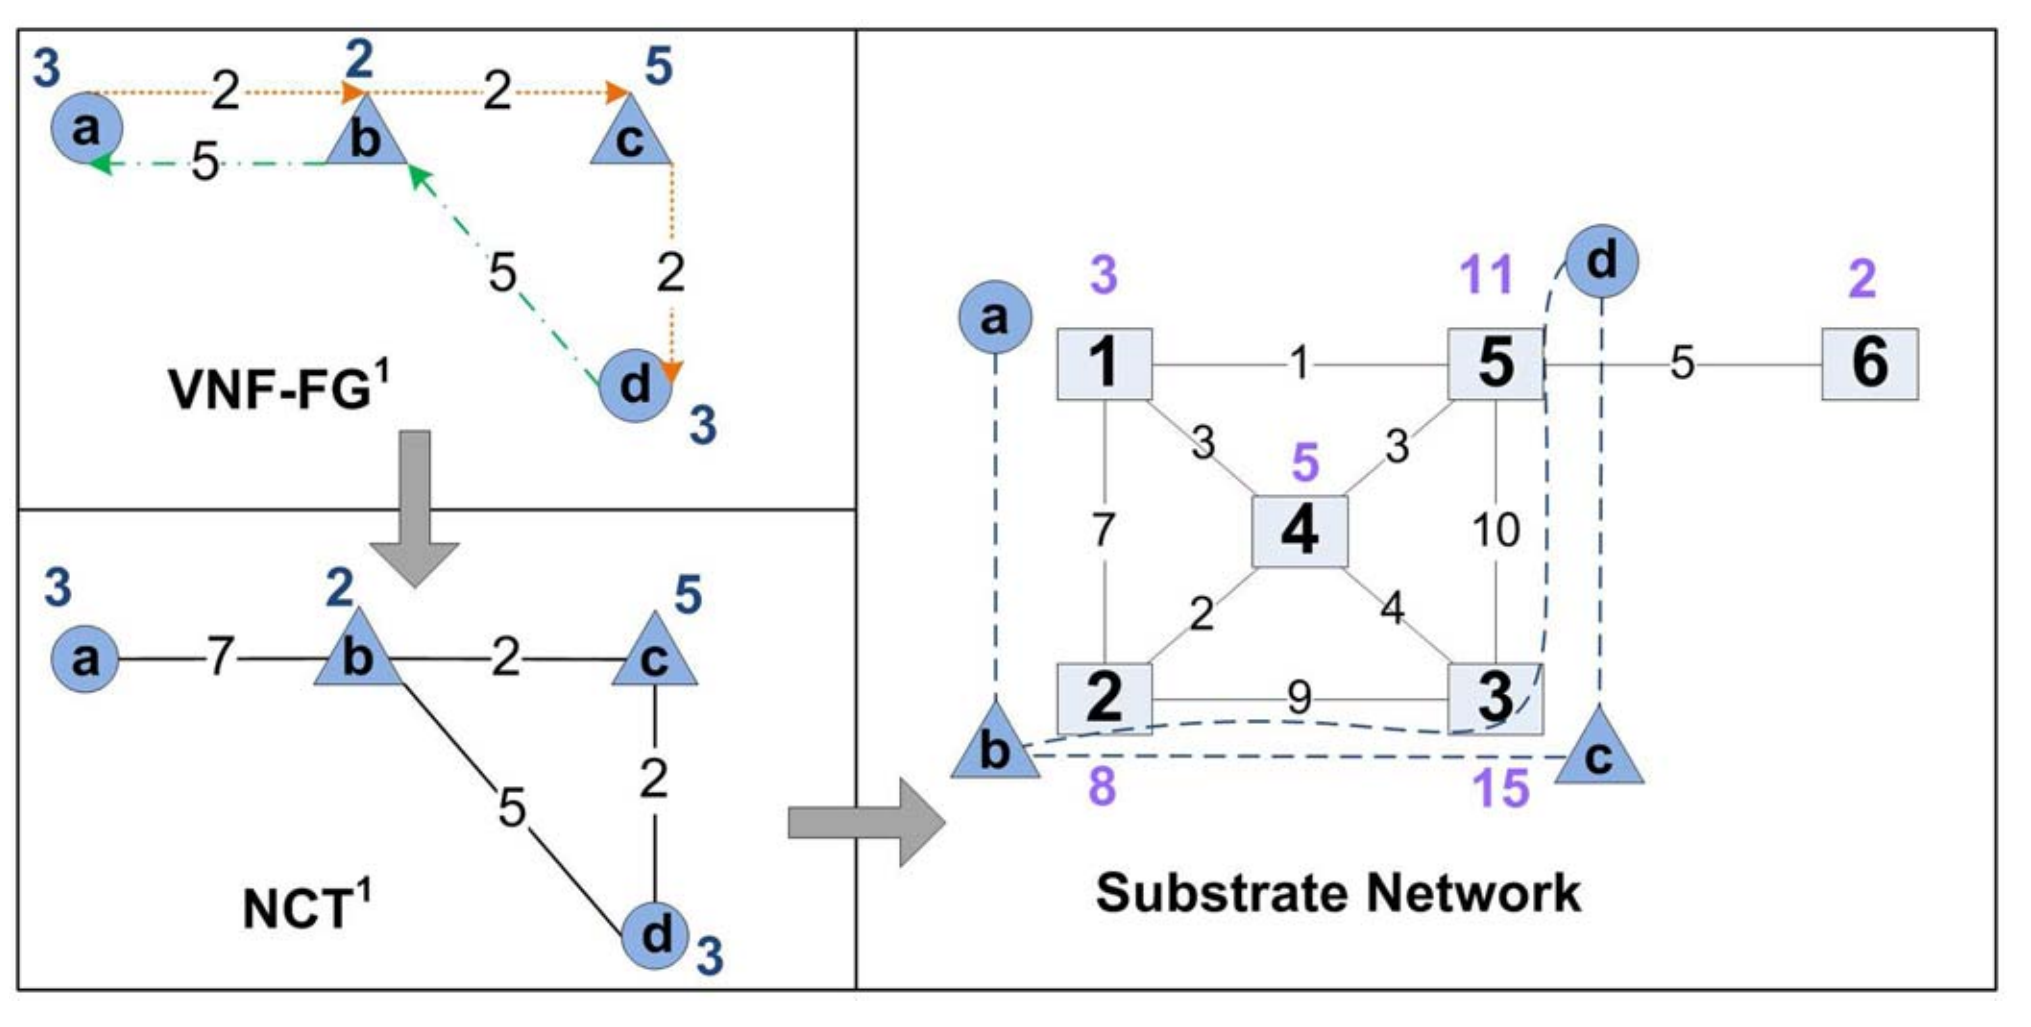
\includegraphics[width = .8\textwidth]{5.png}
    \caption{VNF放置和链接过程图}
    \label{figure:5}
\end{figure}
首先计算任意两个不直接相连的物理节点之间的所有路径上的最小链路带宽的最大值,将计算结果更新为基底图邻接矩阵$A_{SG}$中两个不直接相连的物理节点之间的链路带宽。\par
由于特征分解处理的是相同大小的图,所以需要在请求图中添加虚拟孤立顶点,以使图的大小相等。通过变换大小为m的邻接矩阵$A_{NCT}$,添加n-m行和n-m列的全0向量,使得邻接矩阵$A_{NCT}$的大小为n。\par
如图~\ref{figure:6}所示,以下矩阵分别对应基底图邻接矩阵$A_{SG}$和请求邻接矩阵$A_{NCT}$。\par
\begin{figure}[H]
    \centering
    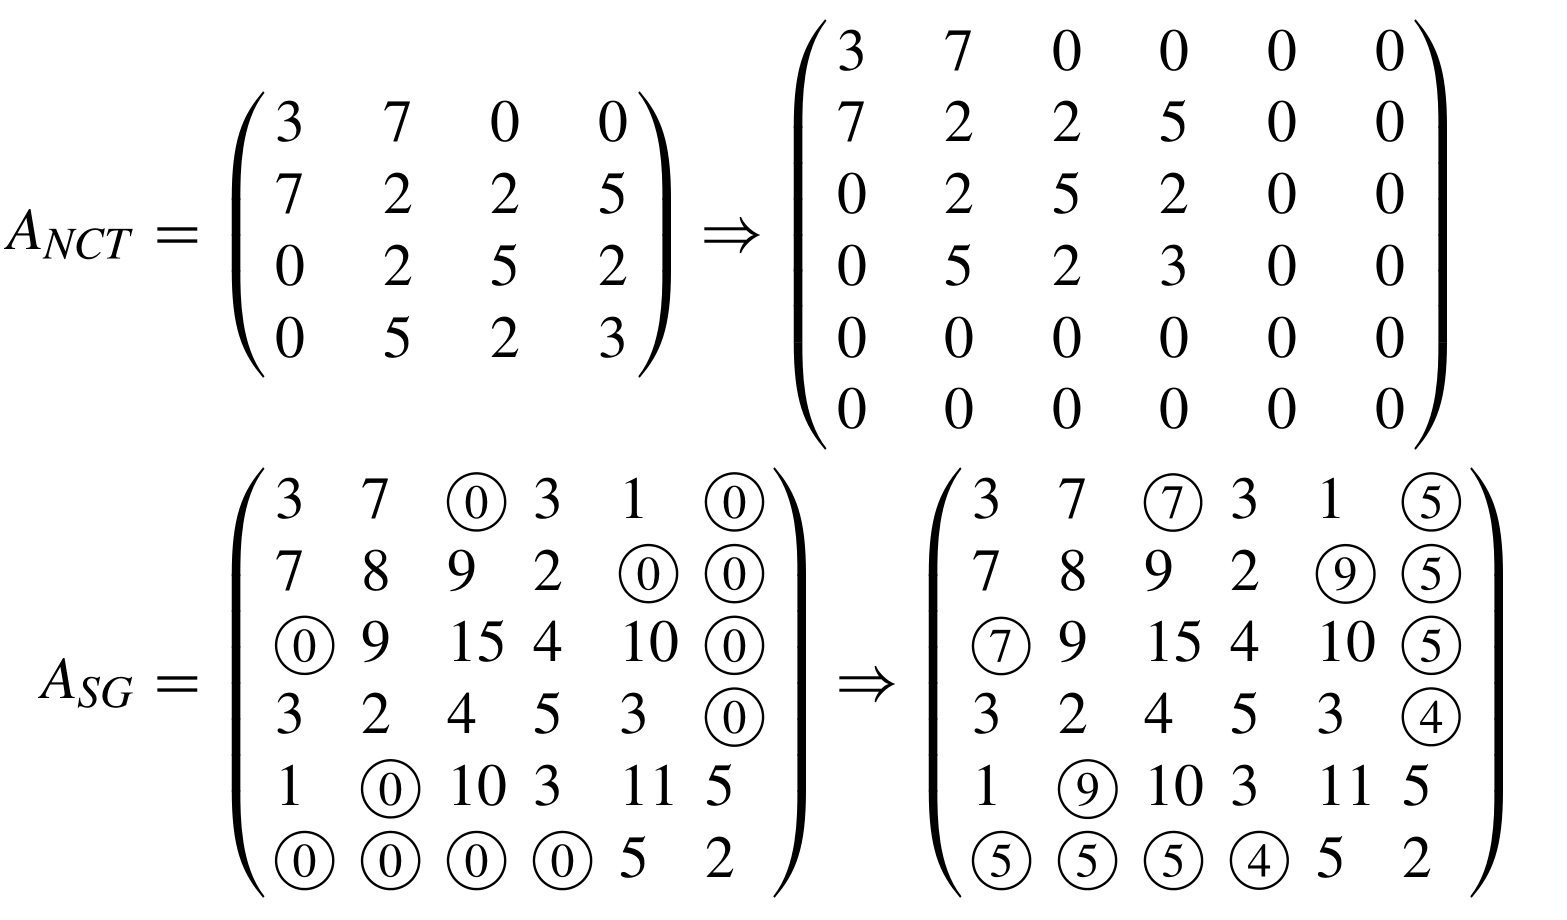
\includegraphics[width = .6\textwidth]{6.png}
    \caption{邻接矩阵图}
    \label{figure:6}
\end{figure}
根据算法1,可以计算出扩展后的$A_{NCT}$矩阵和基底图邻接矩阵$A_{SG}$的特征向量,然后计算出特征向量绝对值的乘积M,结果如图~\ref{figure:7}所示。\par

\begin{algorithm}[H]
    \caption{特征分解算法}
    \begin{algorithmic}[1]
        \STATE 计算任意两个不直接相连的物理节点之间的所有物理路径上的最小链路带宽的最大值\
        \STATE 根据计算结果更新基底图邻接矩阵$A_{SG}$\
        \STATE 计算$A_{SG}$的特征向量矩阵$U_{SG}$\
        \STATE 根据VNF-FG得到网络连接拓扑图NCT\
        \STATE 扩展$A_{NCT}$矩阵使得$A_{SG}$和$A_{NCT}$的矩阵大小相等\
        \STATE 计算$A_{NCT}$的特征向量矩阵$U_{NCT}$\
        \STATE $M\leftarrow \overline{U}_{NCT^c}\times \overline{U}_{SG}^T$\
        \STATE 根据算法2计算出置换矩阵P
    \end{algorithmic}
\end{algorithm}

\begin{figure}[H]
    \centering
    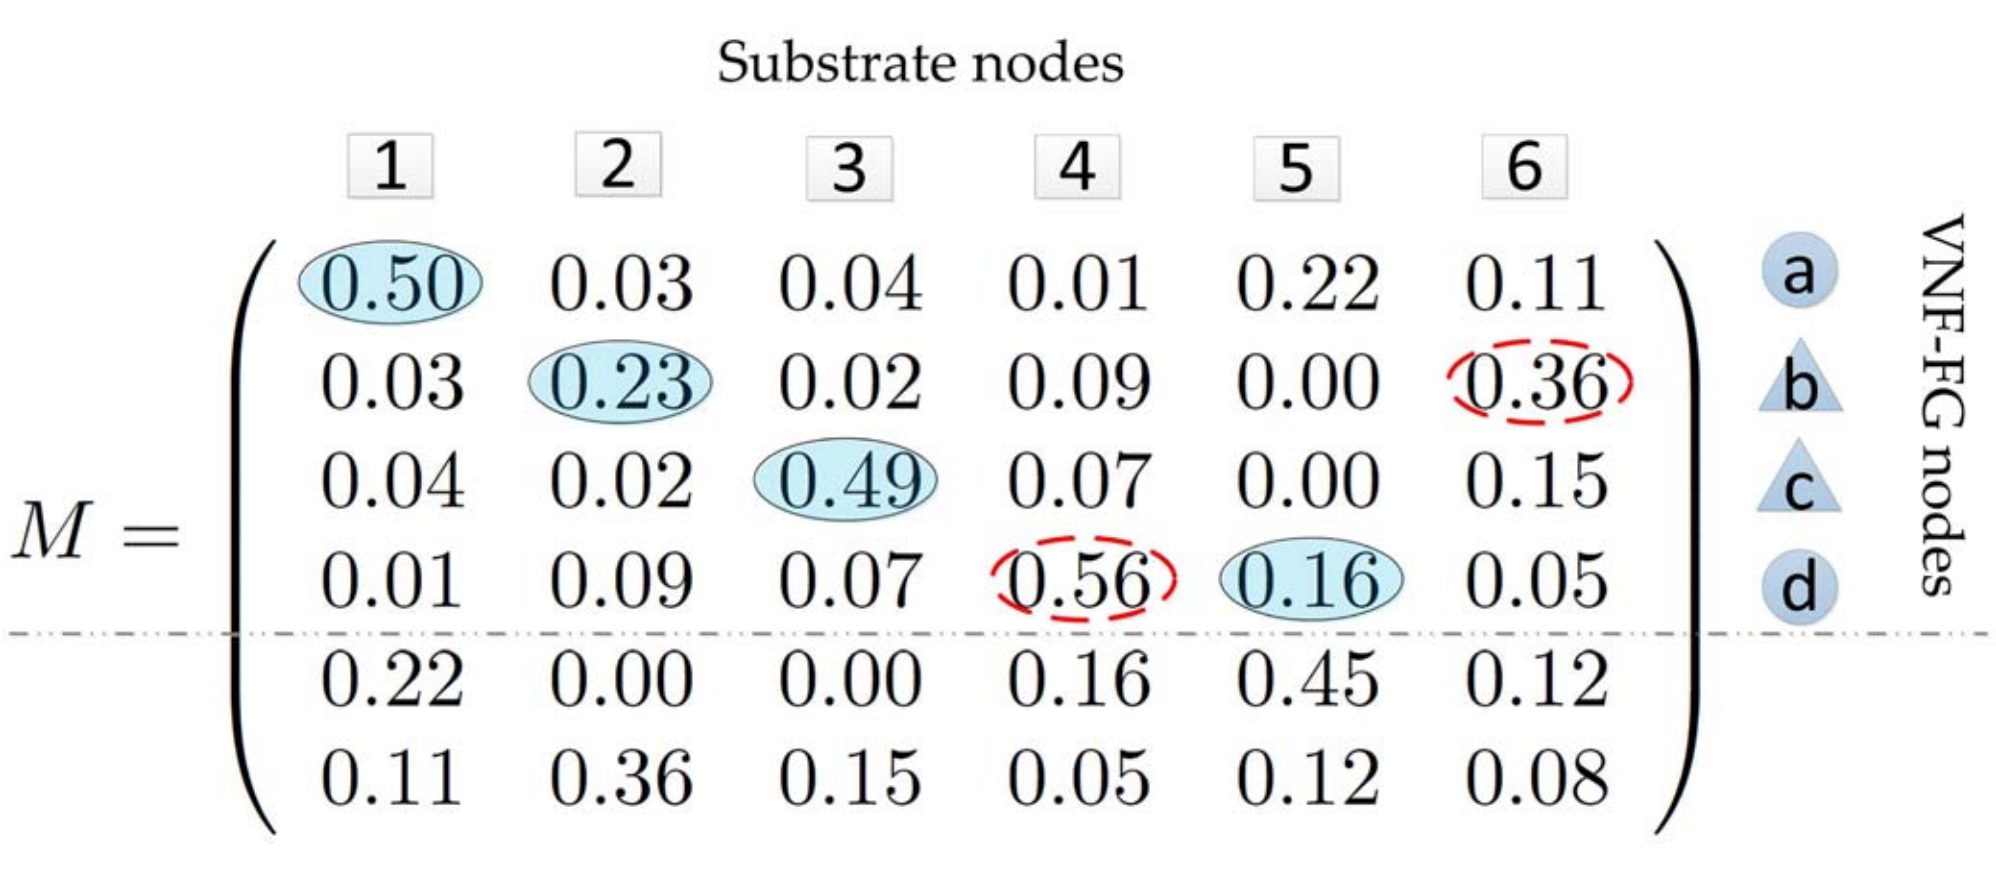
\includegraphics[width = .6\textwidth]{7.png}
    \caption{特征向量乘积计算结果}
    \label{figure:7}
\end{figure}
下一步通过VNF-FG匹配算法来计算出置换矩阵P。对于VNF-FG初始请求的每个VNF,矩阵M中更高的元素值反映了最可能的最佳匹配。这些最可能的匹配需要由算法2进行校验,以验证节点、链路的所有约束条件都得到满足。\par 
\begin{algorithm}[htbp]
    \caption{VFG-FG匹配算法}
    \begin{algorithmic}[1]
    \REQUIRE $NCT^{c}=\left(N^{c}, E^{c}\right) ; S G=\left(N^{s}, E^{s}\right) ; M=\bar{U}_{N C T^{c}} \times \bar{U}_{S G}^{T}$
    \ENSURE  置换矩阵P;VNF-FG最终的放置和扩展结果
    \FOR{each $n_i^c\in N^c$}
    \STATE $Row\leftarrow $矩阵M的第i行
    \STATE $k\leftarrow $计算Row中最大值的下标\
    \IF{$cpu⁡(n_k^s )-cpu⁡(n_i^c)\geq0$ and (其他的节点约束都符合)}
    \IF{CheckLinks ($n_i^c,n_k^s$)= True}
    \STATE$ϕ(n_i^c)\leftarrow n_k^s$\
    \STATE  $P(i,k) \leftarrow 1$\
    \STATE 更新邻接矩阵$A_{SG}$\
    \ELSE
    \STATE $Row[k]\leftarrow null$\
    \STATE Goto Step 3\
    \ENDIF
    \ELSE
    \STATE $Row[k]\leftarrow null$\
    \STATE Goto Step 3\
    \ENDIF
    \ENDFOR\
    \RETURN P\
    % \Function{CHECKLINKS}{$n_i^c,n_k^s$}
    \STATE
    \STATE\textbf{function} CHECKLINKS($n_i^c,n_k^s$)\
    \STATE\quad\textbf{for} each $l \in neighbours(n_i^c)$ 
    \STATE\quad\quad\textbf{if} 节点l已经被放置 \textbf{then}
    \STATE\quad\quad\quad\textbf{if} $[bw(e^s (n_k^s,ϕ(l)))-bw(e^c (n_i^c,l))]<0$ and (符合节点约束) \textbf{then}
    \STATE\quad\quad\quad\quad\textbf{return} False
    \STATE\quad\quad\quad\textbf{end if}
    \STATE\quad\quad\textbf{end if}
    \STATE\quad\textbf{end for}
    \STATE\textbf{end function}
    % \FOR{each $l \in neighbours(n_i^c)$}
    %    \IF{节点l已经被放置}
    %         \IF{$[bw(e^s (n_k^s,ϕ(l)))-bw(e^c (n_i^c,l))]<0$ and (符合节点约束)}
    %             \STATE return False\
    %         \ENDIF
    %     \ENDIF
    % \ENDFOR\
    % \RETURN True\
    
    % \EndFunction
    \end{algorithmic}
\end{algorithm}\par
在置换矩阵P中,成功放置的节点所对应的元素的值会被设置为1。根据算法2计算出的置换矩阵P如图~\ref{figure:8}所示。\par
\begin{figure}[H]
    \centering
    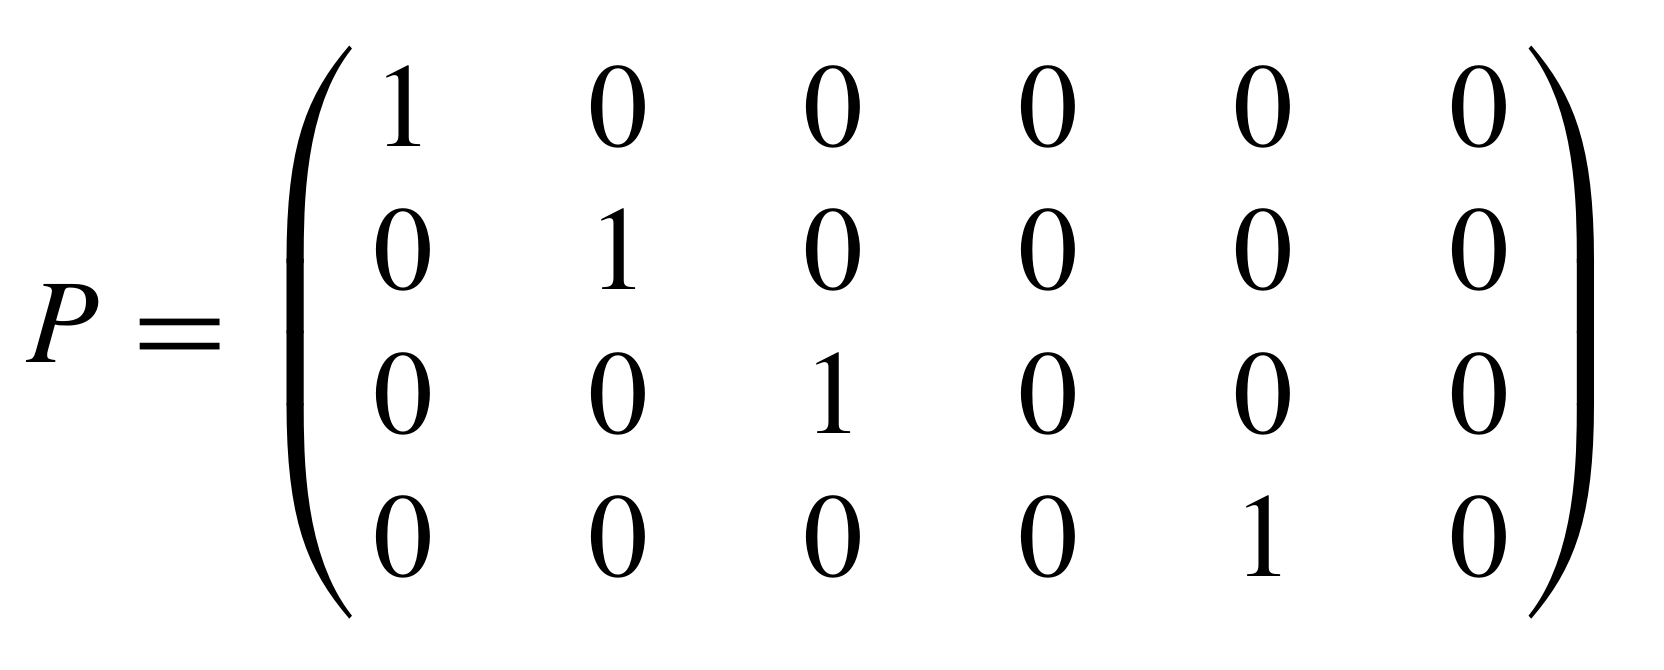
\includegraphics[width=.5\textwidth]{8.png}
    \caption{置换矩阵P}
    \label{figure:8}
\end{figure}

例如,托管所请求的VNF节点b的最可能的候选节点是节点6(值为0.36)。然而,节点6并没有被选中,因为不能符合VNF节点a与b之间链路带宽大于7的要求。节点1和节点6之间的最大可用带宽仅为5。同样,对于放置VNF节点d的候选节点4,尽管在矩阵m中的值更高,但是不能满足链路带宽约束。映射VNF节点b和VNF节点d之间的链路,只有候选节点5满足所有要求(节点2$\rightarrow$节点3$\rightarrow$节点5)。\par
算法2中的步骤1到步骤3,从特征分解算法的角度来匹配最合适的候选节点。M的每一行中的最大的元素值,代表了最佳的节点匹配。步骤4到8用来验证候选节点是否满足整数线性规划模型中设计的所有约束条件。如果候选节点不能满足所有约束条件,算法返回到步骤3,继续验证该元素在矩阵M中的所在行的下一个最大元素值所在节点是否符合所有约束条件。步骤20到28对应于由步骤5调用的函数,该函数用来验证“所选节点及其相邻节点的所有链路”是否都满足约束条件。实际上,算法1中基于特征分解的方法计算出最适合放置VNF节点的物理节点,元素值越大就意味着更合适的节点匹配,但最终的匹配结果由算法2计算得出。\par
算法1和算法2主要解决了VNF-FG的初始放置问题。为了实现扩展,需要在原有算法的基础上,对基底图的邻接矩阵$A_{SG}$进行一些更新,首先需要删除旧图中所利用CPU资源和链路带宽资源,同时固定先前部署的节点在矩阵M中的位置。将旧图中已被放置的物理节点的CPU剩余容量设置为0,避免新的VNF节点放置到已经放置过的物理节点中。新的VNF-FG扩展请求矩阵包括扩展请求的新节点、旧图中与新节点相连接的节点,这些旧的节点需要继续放置在原来的位置,而扩展请求节点不需要受到限制。\par
解决方案的复杂性取决于算法1和算法2的复杂性。NCT和SG的邻接矩阵的特征分解的复杂度直接取决于它们的大小n,并且这个复杂度已知为$O(n^3)$。算法1的步骤8调用了算法2,算法2的算法复杂度应该为$O(m*n*(n-1))$。在算法3的步骤1,涉及到m次循环。在步骤11和步骤15中,在最坏情况下可能会涉及到n次循环。在步骤20中,需要对候选节点的所有邻接节点进行遍历,所以最坏算法复杂度为$O(n-1)$。综上所述,对于我们的解决方案的最坏算法复杂度为$O(n^3)$。\par
特征分解算法是一种在尽可能降低算法复杂度的情况下用于解决VNF-FG扩展问题的算法。在算法2的步骤1中,由于对VNF节点的放置具有一定的特定顺序,导致算法可能计算出局部最优解。同时在算法2中并没有进行回溯,这是因为作为一种启发式算法,在矩阵M中每一行中的最大的元素值就代表着最合适的候选节点,可以更快地计算出符合条件的候选节点。对于VNF节点的顺序进行重新排序和在算法2中进行回溯会使得算法复杂度更高。特征分解算法在更低的算法复杂度和更好的放置结果之间进行了比较好的平衡。\par
\subsubsection{仿真实现}
请求图和物理图都是通过GT-ITM工具和Germany50网络拓扑绘制的。\\
1、模拟环境\par
VNF-FG请求使用泊松过程生成,平均每100个时间单位2个请求。每个请求的生命周期遵循指数分布,距离下一个节点平均时间间隔为50个时间单位。VNF-FG请求模拟分布如图~\ref{figure:9}所示。
\begin{figure}[H]
    \centering
    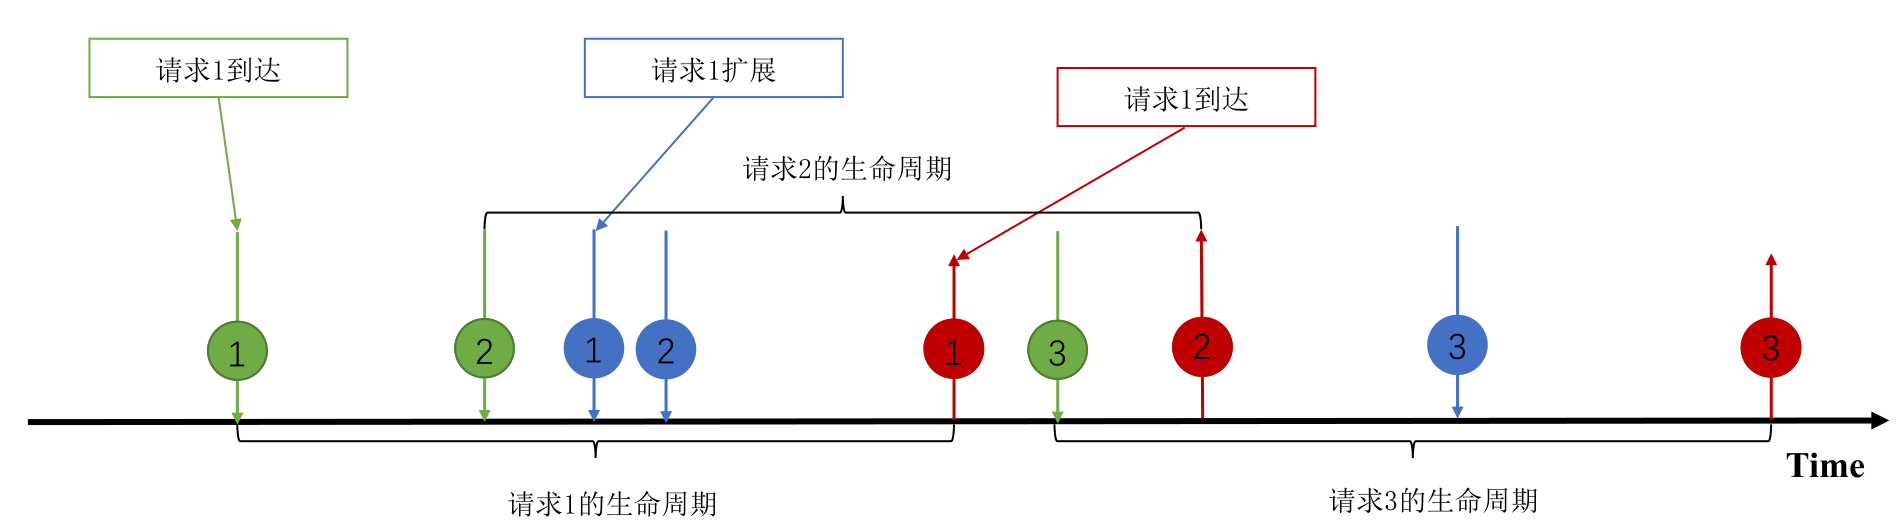
\includegraphics{9.png}
    \caption{VNF-FG请求模拟分布图}
    \label{figure:9}
\end{figure}
物理网络基础设施使用Germany50网络拓扑结构。物理节点和链路的容量在[100,120]的间隔内随机生成。初始VNF-FG请求被设置为4个节点。扩展的请求被设置为3个节点。初始VNF-FG设置为每个虚拟节点10个CPU单元,每个虚拟链路10个单元。扩展VNF-FG设置为每个虚拟节点20个CPU单元,每个虚拟链路20个单元。VNF-FG节点之间的连通性设置为0.3。\\
2、性能指标\par
  1. 成功放置在物理图中的VNF-FG的请求数量;\par
  2. 成功扩展次数与所有生成的VNF-FG请求次数的比率;\par
  3. 执行时间:反映了算法的复杂性。\\
3、仿真结果\par
左图描述了成功放置在物理图中的VNF-FG的请求数量随时间变化的曲线,x轴为时间维度,y轴为扩展请求中成功放置的次数。右图描述了成功扩展次数与所有生成的VNF-FG请求次数的比率随时间变化的曲线,x轴为时间维度,y轴为成功扩展次数与所有生成的VNF-FG请求次数的比率。\\
\begin{figure}[H]
    \centering    %居中
    \subfigure[扩展成功数量]{
    \begin{minipage}[c]{0.5\textwidth}
    \centering
    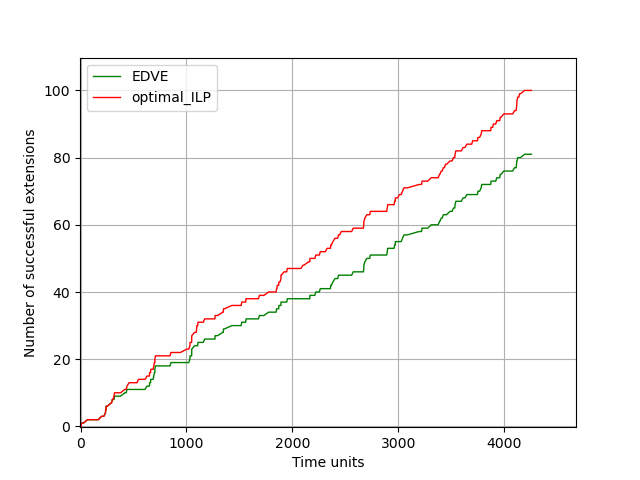
\includegraphics[height=4.5cm,width=7.5cm]{10.png}
    \end{minipage}%
    }%
    \subfigure[扩展成功比率]{
    \begin{minipage}[c]{0.5\textwidth}
    \centering
    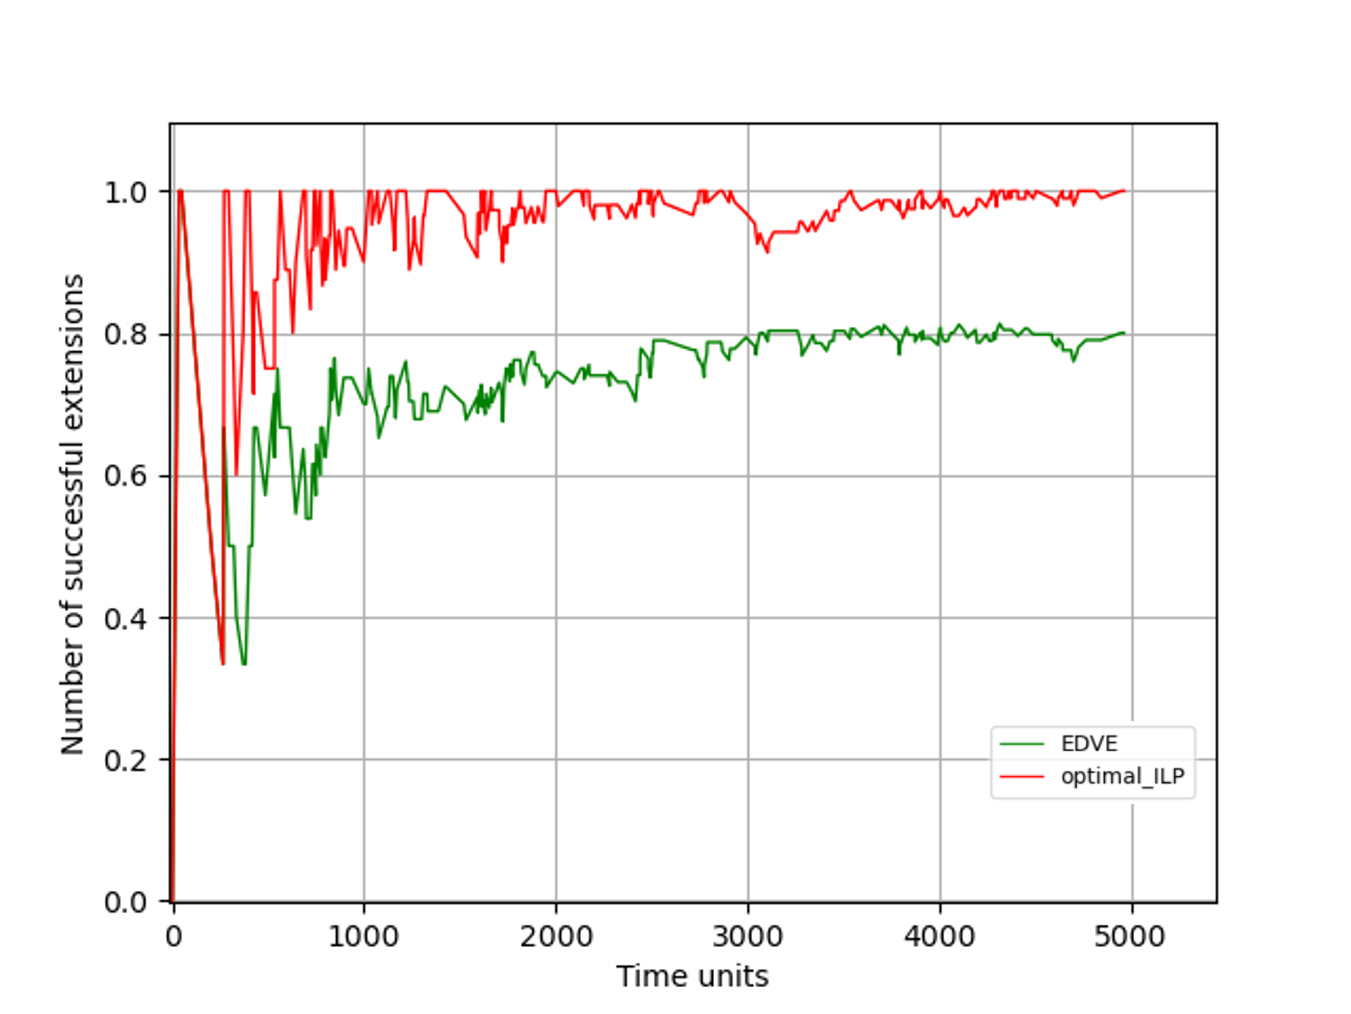
\includegraphics[height=4.5cm,width=7.5cm]{11.png}
    \end{minipage}%
    }%
    \caption{特征分解算法扩展结果图} %  %大图名称
    \label{fig:1}  %图片引用标记
\end{figure}


% \begin{figure}[htbp]
%     \raggedright
%     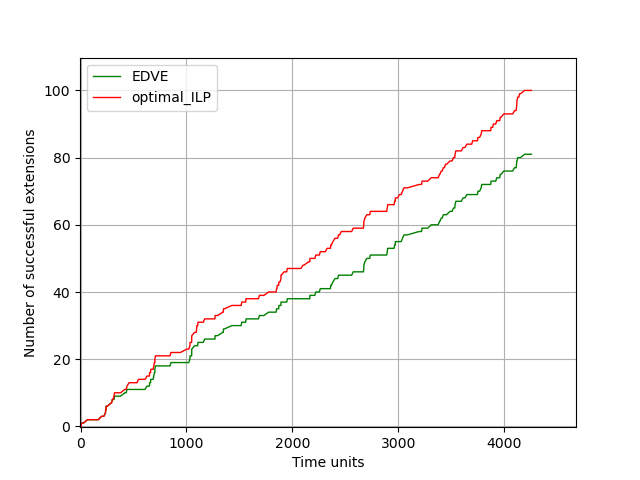
\includegraphics[width=0.5\textwidth]{10.png}
%     \caption{扩展成功数量}
% \end{figure}
% \begin{figure}[htbp]
%     \raggedleft
%     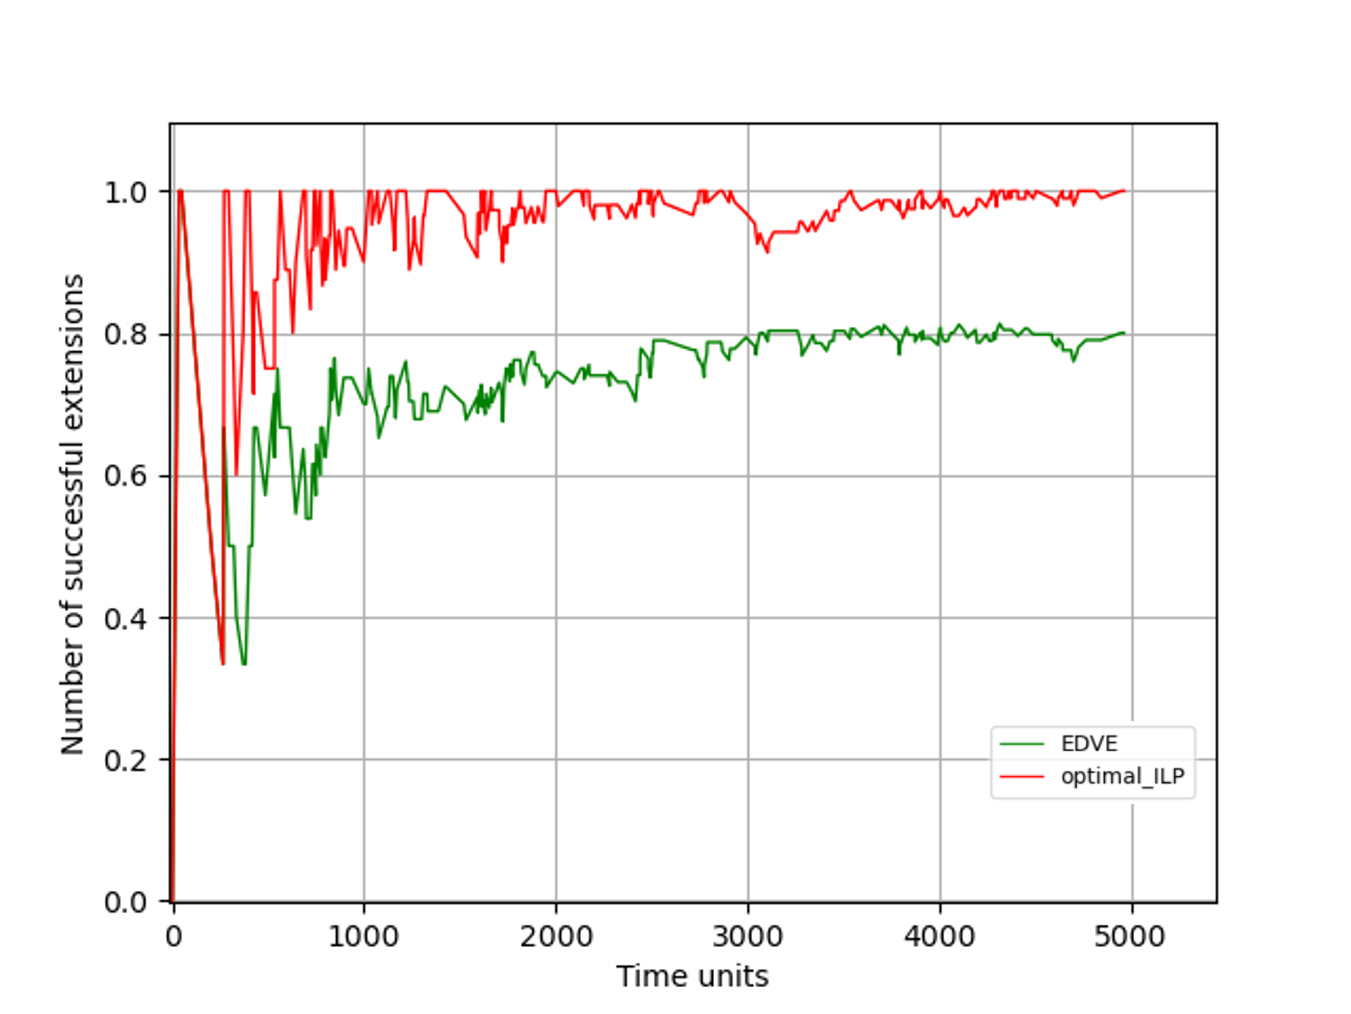
\includegraphics[width=0.5\textwidth]{11.png}
%     \caption{扩展成功比率}
% \end{figure}

图~\ref{figure:12}描述了特征分解算法的扩展结果的目标函数随时间变化的曲线,用于表示所提出的算法的实现质量。在本文中,根据目标函数Z的值定义映射质量,该函数描述了算法在给定的物理网络基础设施上实现负载均衡的能力。\par
\begin{figure}[H]
    \centering
    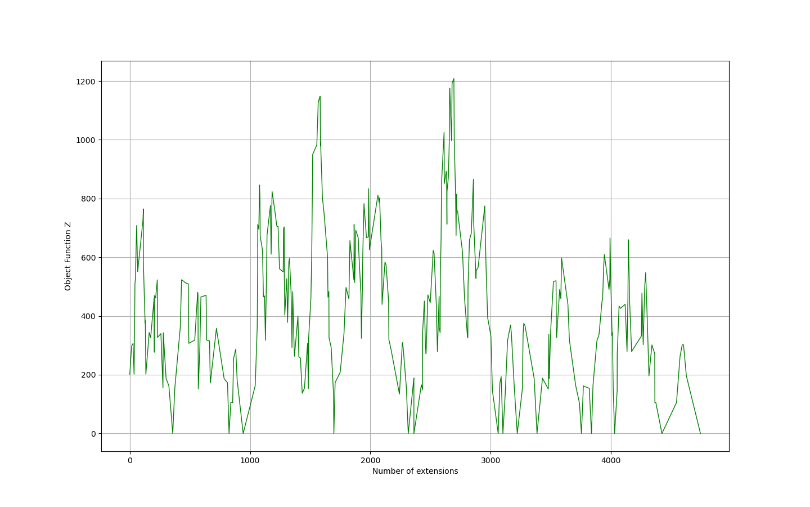
\includegraphics{12.png}
    \caption{目标函数图}
    \label{figure:12}
\end{figure}

\section{后期拟完成的研究工作及进度安排}

\subsection{后期拟完成的研究工作}
\begin{enumerate}
    \setlength{\itemsep}{0pt}
    \setlength{\parsep}{0pt}
    \setlength{\parskip}{0pt}
    \setlength{\topsep}{0pt}
    \setlength{\partopsep}{0pt}
    \item 使用Lingo软件对整数线性规划模型计算最优解;
    \item 对于特征分解算法的仿真实现还存在部分问题没有解决;
    \item 总结课题研究成果,撰写结题报告,准备毕业答辩。
\end{enumerate}
\subsection{后期进度安排}
后期进度安排如表\ref{table:4}所示。
\begin{table}[H]
    \centering
    \caption{进度安排表}
    \label{table:4}
    % \hspace{0.5cm}
    \begin{tabular}{cll}
        \toprule
        序号&研究内容&起止日期\\
        \midrule
        1&解决实现启发式算法实现中存在的问题&2020.04.25-2021.05.05\\
        \midrule
        2&使用Lingo软件对ILP模型计算最优解&2021.05.05-2021.05.15\\
        \midrule
        3&总结研究结果,撰写论文&2021.05.15-2021.05.30\\
        \bottomrule
    \end{tabular}
\end{table}

\section{存在的问题与困难}
\begin{enumerate}
    \setlength{\itemsep}{0pt}
    \setlength{\parsep}{0pt}
    \setlength{\parskip}{0pt}
    \setlength{\topsep}{0pt}
    \setlength{\partopsep}{0pt}
    \item 对于使用Lingo软件对整数线性规划模型进行计算最优解,还存在编程不熟练的问题。
    \item 对于特征分解算法的严格数学证明还存在理解不透彻的问题。
\end{enumerate}
\section{论文按时完成的可能性}
\begin{enumerate}
    \setlength{\itemsep}{0pt}
    \setlength{\parsep}{0pt}
    \setlength{\parskip}{0pt}
    \setlength{\topsep}{0pt}
    \setlength{\partopsep}{0pt}
    \item 目前按照毕业设计开题设计的进度安排,已经如期完成设定的目标。
    \item 毕业设计的大部分工作已经完成,按照进度计划进行,可以按时完成毕业设计。
\end{enumerate}
\section{参考文献}
\begin{thebibliography}{9}
    \bibitem{bibitem1} M. Mechtri, C. Ghribi, and D. Zeghlache, “VNF placement and chain-ing in distributed cloud,” in Proc. 9th IEEE Int. Conf. Cloud Comput.(CLOUD), San Francisco, CA, USA, Jun./Jul. 2016, pp. 376–383.
    \bibitem{bibitem2} Houidi O, Soualah O, Louati W, et al. Dynamic VNF Forwarding Graph Extension Algorithms[J]. IEEE Transactions on Network and Service Management, 2020.
    \bibitem{bibitem3} X. Li and C. Qian, “The virtual network function placement problem,”in Proc. IEEE Conf. Comput. Commun. Workshops, (INFOCOM) Workshops, Hong Kong, Apr./May 2015, pp. 69–70.
    \bibitem{bibitem4} 	O. Houidi, O. Soualah, W. Louati, M. Mechtri, D. Zeghlache, and F. Kamoun, “An efficient algorithm for virtual network function scaling,” in Proc. IEEE Global Commun. Conf. (GLOBECOM), Singapore, Dec. 2017, pp. 1–7.
    \bibitem{bibitem5} S. Dräxler, H. Karl, and Z. Á. Mann, “JASPER: Joint optimization of scaling, placement, and routing of virtual network services,” IEEE Transa. Netw. Serv. Manag., vol. 15, no. 3, pp. 946–960, Sep. 2018.
    \bibitem{bibitem6} 	S. Ayoubi, Y. Zhang, and C. Assi, “A reliable embedding framework for elastic virtualized services in the cloud,” IEEE Transa. Netw. Serv. Manag., vol. 13, no. 3, pp. 489–503, Sep. 2016.
    \bibitem{bibitem7} 	J. Liu, W. Lu, F. Zhou, P. Lu, and Z. Zhu, “On dynamic service function chain deployment and readjustment,” IEEE Transa. Netw. Serv. Manag., vol. 14, no. 3, pp. 543–553, Sep. 2017.
    \bibitem{bibitem8} 	Y. Li, L. T. X. Phan, and B. T. Loo, “Network functions virtualization with soft real-time guarantees,” in Proc. 35th Annu. IEEE Int. Conf. Comput. Commun. (INFOCOM), San Francisco, CA, USA, Apr. 2016, pp. 1–9.
    \bibitem{bibitem9} 	W. Rankothge, F. Le, A. Russo, and J. Lobo, “Optimizing resource allocation for virtualized network functions in a cloud center using genetic algorithms,” IEEE Transa. Netw. Serv. Manag., vol. 14, no. 2, pp. 343–356, Jun. 2017.
    \bibitem{bibitem10} 	Mehraghdam S, Keller M, Karl H. Specifying and Placing Chains of Virtual Network Functions[J]. 2014, 1(1):7-13
    \bibitem{bibitem11} 	Beck M T, Botero J F. Coordinated Allocation of Service Function Chains[C]. Network Function Virtualization and Software Defined Networks. IEEE, 2015, 1-6
    \bibitem{bibitem12} 	Ye Z, Cao X, Wang J, et al. Joint topology design and mapping of service function chains for efficient, scalable, and reliable network functions virtualization[J]. IEEE Network, 2016, 30(3):81-87
    \bibitem{bibitem13} 	Cao J, Zhang Y, An W, et al. VNF-FG design and VNF placement for 5G mobile networks[J]. Science China, 2017, 60(4):2-5
    \bibitem{bibitem14} 	Sun Q, Lu P, Lu W, et al. Forecast-Assisted NFV Service Chain Deployment Based on Affiliation-Aware vNF Placement[C]. Global Communications Conference. IEEE, 2017, 1-9
    \bibitem{bibitem15} 	Houidi O, Soualah O,Louati W, et al. Dynamic VNF Forwarding Graph Extension Algorithms[J]. IEEE Transactions on Network and Service Management, 2020.
    \bibitem{bibitem16} Mijumbi R,Serrat J,Gorricho J L,et al. Network function virtualization: State-of-the-art and research challenges[J]. IEEE Communications surveys \& tutorials, 2015, 18(1): 236-262.
    \bibitem{bibitem17} 	Yi B,Wang X,Li K,et al.A comprehensive survey of network function virtualization [J]. Computer Networks, 2018, 133: 212-262.
    \bibitem{bibitem18} 	Kreutz D, Ramos F M V, Verissimo P E, et al. Software-defined networking: A comprehensive survey[J]. Proceedings of the IEEE, 2014, 103(1): 14-76.
    \bibitem{bibitem19} 	Li Y, Chen M. Software-defined network function virtualization: A survey[J]. IEEE Access, 2015, 3: 2542-2553.
    \bibitem{bibitem20} 	Nunes B A A, Mendonca M, Nguyen X N, et al. A survey of software-defined networking: Past, present, and future of programmable networks[J]. IEEE Communications surveys \& tutorials, 2014, 16(3): 1617-1634.
    \bibitem{bibitem21} 	UMEYAMA S. An eigendecomposition approach to weighted graph matching problems[J]. Pattern Analysis \& Machine Intelligence IEEE Transactions on, 1988, 10(5):695-703.
    \bibitem{bibitem22} 	周伟林. 可扩展VNF放置的算法研究与实现[D].北京邮电大学,2019.
    \bibitem{bibitem23} 	周廷枢. 虚拟网络功能转发图设计及映射研究[D].电子科技大学,2018.
    \bibitem{bibitem24} 	邵维专,吕光宏.网络功能虚拟化资源配置及优化研究综述[J].计算机应用研究,2018,35(02):321-326.
\end{thebibliography}
\bibliographystyle{hithesis}
\bibliography{reference}

% Local Variables:
% TeX-master: "../mainart"
% TeX-engine: xetex
% End: